% !TEX TS-program = pdflatex
% !TEX encoding = UTF-8 Unicode

\documentclass[a4paper, titlepage=false, parskip=full-, 10pt]{scrartcl}

\usepackage[utf8]{inputenc}
\usepackage[T1]{fontenc}
\usepackage[english, ngerman]{babel}
\usepackage{babelbib}
\usepackage{hyperref}
\usepackage{listings}
\usepackage{framed}
\usepackage{color}
\usepackage{graphicx}
\usepackage[normalem]{ulem}
\usepackage{cancel}
\usepackage{array}
\usepackage{amsmath}
\usepackage{amssymb}
\usepackage{amsthm}
\usepackage{algorithm}
\usepackage{algorithmic}
\usepackage{geometry}
\usepackage{subfigure}
\geometry{a4paper, top=20mm, left=35mm, right=25mm, bottom=40mm}

\newcounter{tasknbr}
\setcounter{tasknbr}{1}
\newenvironment{task}[1]{{\bf Aufgabe \arabic {tasknbr}\stepcounter{tasknbr}} (#1):\begin{enumerate}}{\end{enumerate}}
\newcommand{\subtask}[1]{\item[#1)]}

% Listings -----------------------------------------------------------------------------
\definecolor{red}{rgb}{.8,.1,.2}
\definecolor{blue}{rgb}{.2,.3,.7}
\definecolor{lightyellow}{rgb}{1.,1.,.97}
\definecolor{gray}{rgb}{.7,.7,.7}
\definecolor{darkgreen}{rgb}{0,.5,.1}
\definecolor{darkyellow}{rgb}{1.,.7,.3}
\lstloadlanguages{C++,[Objective]C,Java}
\lstset{
escapeinside={§§}{§§},
basicstyle=\ttfamily\footnotesize\mdseries,
columns=fullflexible,
keywordstyle=\bfseries\color{blue},
commentstyle=\color{darkgreen},      
stringstyle=\color{red},
numbers=left,
numberstyle=\ttfamily\scriptsize\color{gray},
breaklines=true,
showstringspaces=false,
tabsize=4,
captionpos=b,
float=htb,
frame=tb,
frameshape={RYR}{y}{y}{RYR},
rulecolor=\color{black},
xleftmargin=15pt,
xrightmargin=4pt,
aboveskip=\bigskipamount,
belowskip=\bigskipamount,
backgroundcolor=\color{lightyellow},
extendedchars=true,
belowcaptionskip=15pt}

%% Enter current values here: %%
\newcommand{\lecture}{Robotik WS15/16}
\newcommand{\tutor}{}
\newcommand{\assignmentnbr}{12}
\newcommand{\students}{Julius Auer, Thomas Tegethoff}
%%-------------------------------------%%

\begin{document}  
{\small \textsl{\lecture \hfill \tutor}}
\hrule
\begin{center}
\textbf{Übungsblatt \assignmentnbr}\\
[\bigskipamount]
{\small \students}
\end{center}
\hrule

\begin{task}{}
\subtask{a}
Gesucht sind die Parameter $a,b,c,d,h,i,j,k$ für zwei Splines $f:\mathopen[0,1\mathclose]\rightarrow\mathbb{R} ,g:\mathopen[1,2\mathclose]\rightarrow\mathbb{R}$. Die gesuchten Funktionen mit ihren Ableitungen sind:

\begin{align*}
f(x)&=a\cdot x^3+b\cdot x^2+c\cdot x+d\\
f'(x)&=3\cdot a\cdot x^2+2\cdot b\cdot x+c	\\
f''(x)&=6\cdot a\cdot x+2\cdot b\\
g(x)&=h\cdot x^3+i\cdot x^2+j\cdot x+k\\
g'(x)&=3\cdot h\cdot x^2+2\cdot i\cdot x+j	\\
g''(x)&=6\cdot h\cdot x+2\cdot i
\end{align*}

Aus der Beschreibung sind direkt die folgenden Eigenschaften abzulesen:

\begin{align*}
f(0)&=0\\
f'(0)&=0\\
g(2)&=8\\
g'(2)&=8\\
f''(1)&=0\\
g''(1)&=0
\end{align*}

Um das soweit unterbestimmte Gleichungssystem lösen zu können, verwenden wir als zusätzliche Eigenschaft die Tatsache, dass sich $f$ und $g$ an der Grenze ihrer Definitionsbereiche bei $x=1$ schneiden müssen. Es gilt also zusätzlich:

\begin{align*}
f(1)&=g(1)\\
f'(1)&=g'(1)
\end{align*}

Ausformuliert erhält man somit ein lineares Gleichungssystem:

\begin{align*}
d&=0\\
k&=0\\
8\cdot h+4\cdot i+2\cdot j&=8\\
12\cdot h+4\cdot i+j&=8\\
6\cdot a+2\cdot b&=0\\
6\cdot h+2\cdot i&=0\\
a+b+c&=h+i+j\\
3\cdot a+2\cdot b+c&=3\cdot h+2\cdot i+j
\end{align*}

$d,k$ sind also an dieser Stelle bereits bekannt. Für die übrigen Parameter lösen wir mittels Gaussschem Eliminierungsverfahren (*stöhn*):

\begin{center}\begin{tabular}{cccccc|c}
$a$&$b$&$c$&$h$&$i$&$j$&$=$\\\hline
0&0&0&8&4&2&8\\
0&0&0&12&4&1&8\\
6&2&0&0&0&0&0\\
0&0&0&6&2&0&0\\
1&1&1&-1&-1&-1&0\\
3&2&1&-3&-2&-1&0
\end{tabular}\end{center}

Zuerst etwas umsortieren:

\begin{center}\begin{tabular}{cccccc|c}
$a$&$b$&$c$&$h$&$i$&$j$&$=$\\\hline
1&1&1&-1&-1&-1&0\\
3&2&1&-3&-2&-1&0\\
6&2&0&0&0&0&0\\
0&0&0&6&2&0&0\\
0&0&0&8&4&2&8\\
0&0&0&12&4&1&8
\end{tabular}\end{center}

$a$-Spalte eliminieren:

\begin{center}\begin{tabular}{cccccc|c}
$a$&$b$&$c$&$h$&$i$&$j$&$=$\\\hline
1&1&1&-1&-1&-1&0\\
0&-1&-2&0&1&2&0\\
0&-4&-6&6&6&6&0\\
0&0&0&6&2&0&0\\
0&0&0&8&4&2&8\\
0&0&0&12&4&1&8
\end{tabular}\end{center}

$b$-Spalte eliminieren:

\begin{center}\begin{tabular}{cccccc|c}
$a$&$b$&$c$&$h$&$i$&$j$&$=$\\\hline
1&1&1&-1&-1&-1&0\\
0&1&2&0&-1&-2&0\\
0&0&2&6&2&-2&0\\
0&0&0&6&2&0&0\\
0&0&0&8&4&2&8\\
0&0&0&12&4&1&8
\end{tabular}\end{center}

$c$-Spalte sieht schon gut aus, deshalb weiter mit $h$:

\begin{center}\begin{tabular}{cccccc|c}
$a$&$b$&$c$&$h$&$i$&$j$&$=$\\\hline
1&1&1&-1&-1&-1&0\\
0&1&2&0&-1&-2&0\\
0&0&1&3&1&-1&0\\
0&0&0&6&2&0&0\\
0&0&0&0&4&6&24\\
0&0&0&0&0&1&8
\end{tabular}\end{center}

So ein Glück: $i,j$ ergeben sich direkt! Von unten nach oben können nun alle Parameter ausgerechnet werden, zu:

\begin{align*}
&a=2,b=-6,c=8,\\
&h=2,i=-6,j=8
\end{align*}

Eine partielle Interpolation war hier also gar nicht nötig - ein einziges Polynom $e:\mathopen[0,2\mathclose]\rightarrow\mathbb{R}$ genügt,
um alle Eigenschaften zu erfüllen. Ergebnis:

$$e(x)=2\cdot x^3-6\cdot x^2+2\cdot x$$

\subtask{b}
Auch wenn $f=g=e$ sind hier unabhängig von einander $f$ in blau und $g$ in rot geplottet (Abbildung \ref{fig:1}).

\begin{figure}[!htpb]
\centering
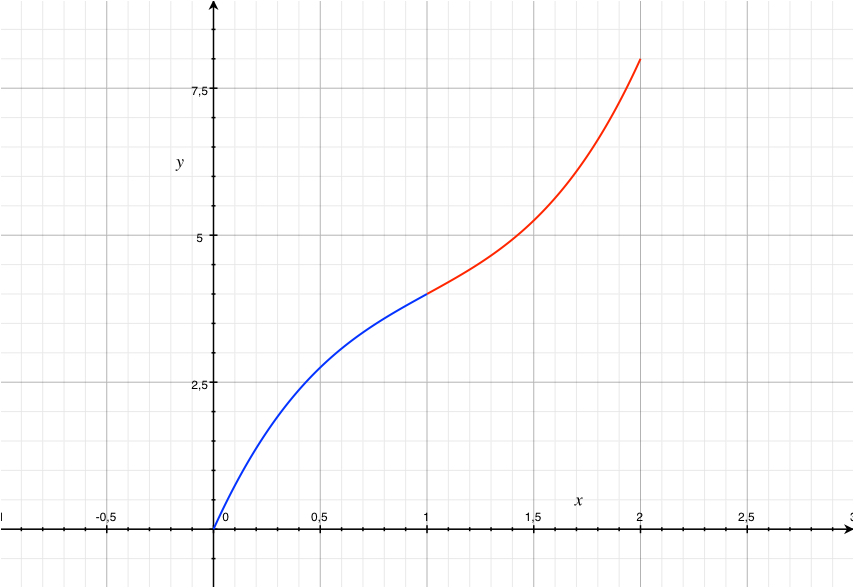
\includegraphics[width=\linewidth]{capture_1-1}
\caption{Spline}
\label{fig:1}
\end{figure}

\subtask{c}
Der Schnittpunkt $(x_s,y_s)$ ist vorgegeben bei $x_s=1$ mit:

$$y_s=e(1)=a+b+c=4$$

Die Geschwindigkeit $v$ ist dort:

$$v=e'(1)=3\cdot a+2\cdot b+c=2$$
\end{task}

\newpage
\begin{task}{}
\item[]
Es muss nur ein klitzekleines Stückchen Code geändert werden, um die zufälligen Punkte zu erzeugen:

\lstinputlisting[language=C++, firstline=46, lastline=56]{../../src/spline_test/src/spline_test.cpp}

Davon abgesehen müssen nur ein paar Grenzen angepasst werden und man erhält Abbildung \ref{fig:2}. Wie genau die Ableitungen am Anfang und am Ende gewählt werden ist letztlich egal (bei uns: $=1$). Code verstanden: check!

\begin{figure}[!htpb]
\centering
\subfigure[$sampling\_num=10$]
{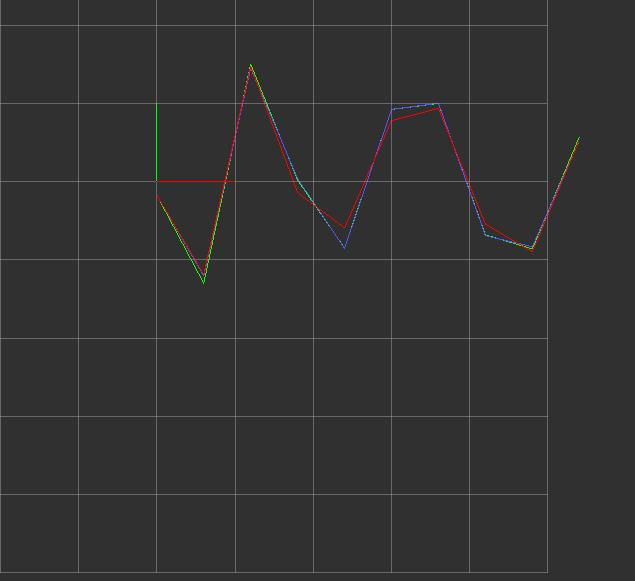
\includegraphics[width=0.8\linewidth]{capture_2-1}}
\subfigure[$sampling\_num=200$]
{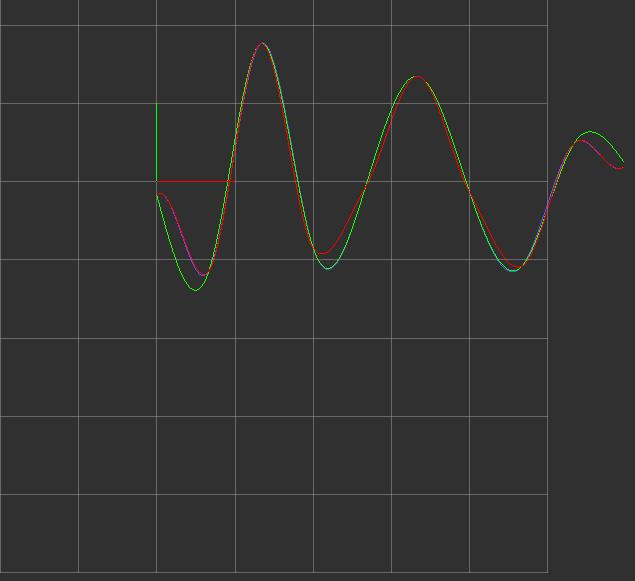
\includegraphics[width=0.8\linewidth]{capture_2-2}}
\caption{Splines}
\label{fig:2}
\end{figure}
\end{task}

\newpage
\begin{task}{}
\subtask{a}
Wir definieren Ereigniss $E$ als ''Enten sind zu sehen'' und Ereigniss $K$ als ''Krokodile sind zu sehen''.

Wir wissen aus der Problembeschreibung:

\begin{align*}
p(E|K)&=0.1\\
p(E|\lnot K)&=0.5\\
p(K)&=0.2
\end{align*}

Um $p(K|\lnot E)$ auszurechnen benötigt man den Satz von Bayes $p(K|\lnot E)=\frac{p(E|\lnot K)\cdot p(K)}{p(\lnot E)}$ und somit noch $p(\lnot E)$. Dieses wiederum ergibt sich aus:

\begin{align*}
p(\lnot E)&=1-p(E)\\
&=1-(p(E|K)+p(E|\lnot K))\\
&=1-0.1-0.5\\
&=0.4
\end{align*}

Eingesetzt in Bayes Satz erhält man so:

\begin{align*}
p(K|\lnot E)&=\frac{p(E|\lnot K)\cdot p(K)}{p(\lnot E)}\\
&=\frac{0.5\cdot 0.2}{0.4}\\
&=0.25
\end{align*}

\subtask{b}
Die Ereignisse $E$ und $K$ sind abhängig. Beweis durch Widerspruch: Angenommen $A$ und $K$ sind unabhängig, dann gilt $P(E|K) = P(E)$. Aber: $0.1\neq 0.6$.\\
\begin{align*}&&&&\qed\end{align*}
\end{task}
\end{document}
